\let\negmedspace\undefined
\let\negthickspace\undefined
\documentclass[journal]{IEEEtran}
\usepackage[a5paper, margin=10mm, onecolumn]{geometry}
%\usepackage{lmodern} % Ensure lmodern is loaded for pdflatex
\usepackage{tfrupee} % Include tfrupee package

\setlength{\headheight}{1cm} % Set the height of the header box
\setlength{\headsep}{0mm}     % Set the distance between the header box and the top of the text

\usepackage{gvv-book}
\usepackage{gvv}
\usepackage{cite}
\usepackage{amsmath,amssymb,amsfonts,amsthm}
\usepackage{algorithmic}
\usepackage{graphicx}
\usepackage{textcomp}
\usepackage{xcolor}
\usepackage{txfonts}
\usepackage{listings}
\usepackage{enumitem}
\usepackage{mathtools}
\usepackage{gensymb}
\usepackage{comment}
\usepackage[breaklinks=true]{hyperref}
\usepackage{tkz-euclide} 
\usepackage{listings}
% \usepackage{gvv}                                        
\def\inputGnumericTable{}                                 
\usepackage[latin1]{inputenc}                                
\usepackage{color}                                            
\usepackage{array}                                            
\usepackage{longtable}                                       
\usepackage{calc}                                             
\usepackage{multirow}                                         
\usepackage{hhline}                                           
\usepackage{ifthen}                                           
\usepackage{lscape}
\begin{document}

\bibliographystyle{IEEEtran}
\vspace{3cm}

\title{9-9.2-20}
\author{EE24BTECH11066 - YERRA AKHILESH
}
% \maketitle
% \newpage
% \bigskip
{\let\newpage\relax\maketitle}

\renewcommand{\thefigure}{\theenumi}
\renewcommand{\thetable}{\theenumi}
\setlength{\intextsep}{10pt} % Space between text and floats


\numberwithin{equation}{enumi}
\numberwithin{figure}{enumi}
\renewcommand{\thetable}{\theenumi}
\textbf{Question}:\\
Find the area of the region bounded by the curves $y = x2 + 2$, $y = x$, $x = 0$ and $x = 3$.
\\
\textbf{solution: }
\begin{table}[h!]
    \centering
    \begin{tabular}[12pt]{ |c| c|}
    \hline
    \textbf{M} & $\nu$ \textbf{(Prandtl-Meyer function)}\\ 
    \hline
    1.8 & 20.73 \\
    \hline
    1.9 & 23.59 \\
    \hline
    2.0 & 26.38 \\
    \hline
    2.1 & 29.10 \\
    \hline
    2.2 & 31.73 \\
    \hline
    2.3 & 34.28 \\
    \hline
    2.4 & 36.75 \\
    \hline
    \end{tabular}
\end{table}
The parameters of the conic are\\
\begin{table}[h!]
    \centering
    \begin{tabular}[12pt]{ |c| c|}
    \hline
    \textbf{Conic}& \textbf{Parameters}\\ 
    \hline
     $V$& $\myvec{0 & 0 \\ 0 & 1}$\\
    \hline 
     $u$& $\frac{-1}{2}\myvec{1\\0}$\\
    \hline
     $f$& $0$\\
     \hline
    \end{tabular}
    \label{Table2}
\end{table}

\begin{align}
    L : x_i=h+\kappa_i m 
\end{align}
Where,
\begin{align}
    \kappa_i=\frac{1}{m^\top Vm}(-m^\top(Vh+u) \pm \sqrt{[m^\top(Vh+u)]^2-g(h)(m^\top Vm)})
    \label{0.2}
\end{align}
For the curves \(y = x^2 + 2\) and \(y = x\), we find the points of intersection by solving
\begin{align}
    x^2 + 2 = x
\end{align}
Rearranging the equation:
\begin{align}
    x^2 - x + 2 = 0
\end{align}
Since this quadratic has no real roots, we calculate the area between the curves over the interval \(x = 0\) to \(x = 3\).

The area between the curves is given by:
\begin{align}
    A = \int_{0}^{3} (x - (x^2 + 2)) \, dx
\end{align}
Simplifying the integrand:
\begin{align}
    A = \int_{0}^{3} (x - x^2 - 2) \, dx
\end{align}
Solving the integral:
\begin{align}
    A = \left[\frac{x^2}{2} - \frac{x^3}{3} - 2x\right]_{0}^{3}
\end{align}
Evaluating at the bounds:
\begin{align}
    A = \left[\frac{9}{2} - \frac{27}{3} - 6 \right] - \left[0\right]
\end{align}
Simplifying:
\begin{align}
    A = \frac{9}{2} - 9 - 6 = \frac{9}{2} - 15 = \frac{-21}{2}
\end{align}
Taking the absolute value, the area of the region is:
\begin{align}
    A = \frac{21}{2}
\end{align}
\begin{figure}[htp]
    \centering
    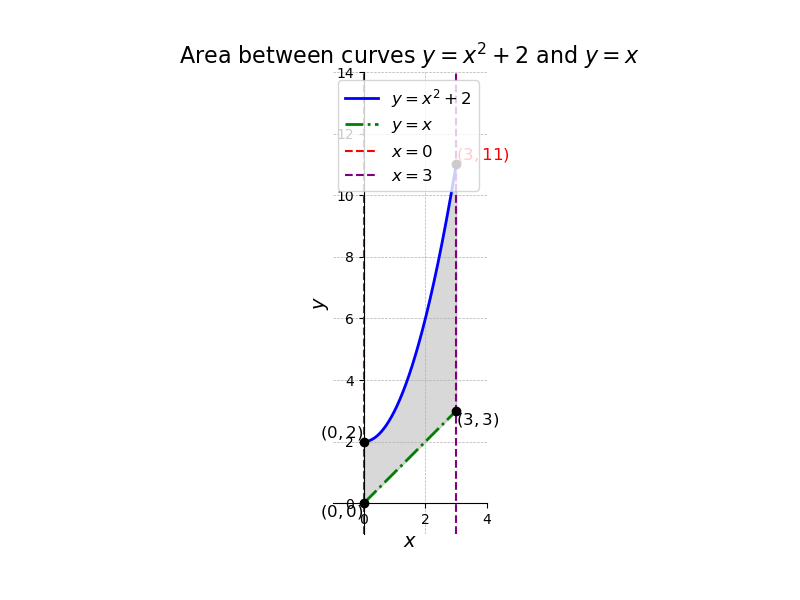
\includegraphics[width=10cm]{figs/Figure_1.png}
\end{figure}
\end{document}










